\clearpage
\section{Related Work}

\subsection{Navigation by Contact and Tactile SLAM}

In highly cluttered or signal-denied environments, traditional collision-avoidance algorithms demand significant computational overhead and rely on heavy optical or LiDAR sensors that frequently fail in feature-poor spaces. While Simultaneous Localization and Mapping (SLAM) remains an active research frontier, reliably deploying it on small, payload-constrained drones in unstructured environments remains an open challenge~\cite{macariorojas2021}. Even state-of-the-art autonomous ground vehicles equipped with expensive sensors and substantial compute have not fully solved reliable real-time navigation in arbitrary environments; the task is substantially harder for a small aerial vehicle.

The constraint of navigating these spaces safely motivates a fundamentally different approach. Mulgaonkar et al.~\cite{mulgaonkarRobustAerialRobot2018} demonstrated that swarms of 25\,g micro-drones could navigate blind environments by intentionally colliding with obstacles and recovering from the impact, rather than detecting and avoiding them. This inverts the traditional SLAM paradigm: instead of building a map to avoid obstacles, the environment is explored through physical contact.

Furthermore, the ability to estimate contact state and impact forces using onboard odometry---termed \emph{contact-inertial odometry}---has been demonstrated to sustain state estimation during collisions by generating pseudo-measurements from external force estimates~\cite{de_petris_collision_2022}. This capability is directly relevant to aerial physical interaction and manipulation (APhI), where Reinforcement Learning (RL) policies must contend with contact dynamics that are difficult to model mathematically, complicating the construction of realistic training environments and reward functions~\cite{borgherini_oneshot_2025}. Recent work has attempted to bridge this gap via inner-loop dynamics estimators that compensate for unmodeled interaction forces within the RL framework~\cite{singh_reinforcement_2026}, underscoring the need for accurate force-feedback estimates of the kind that contact-inertial odometry can provide.

\subsection{Collision-Resilient Drone Designs}

Scaling this collision-resilience concept from 25\,g disposable swarms to a platform capable of carrying inspection sensors and a companion computer introduces a size-dependent penalty. At the 4-inch propeller class, the ratio of inertia to structural strength decreases, and obstacles that a micro-drone's simple tube cage could deflect become proportionally larger relative to the airframe. The protective cage must shield the propellers and fuselage from corners, shelves, and continuous piping---geometries that a minimal cage cannot deflect.

To manage this kinetic penalty, a significant portion of the literature has focused on energy absorption through structural compliance, utilising tensegrity structures~\cite{zhaDesignControlCollisionresilient2023}, arthropod-inspired elastic exoskeletons~\cite{azambujaWhenBeingSoft2022}, and shape-memory origami guards~\cite{parkOrigamiKirigamiStructure2023}. However, these compliant designs often introduce aerodynamic instability or scale poorly to standard industrial inspection platforms.

A more mechanically straightforward approach involves rigid, protective cages that physically decouple the drone's attitude from the collision surface. To ensure self-righting after ground impacts, Mulgaonkar et al.~\cite{mulgaonkarRobustAerialRobot2018} utilised G\"omb\"oc-shaped shells---a convex mono-monostatic body with a single stable equilibrium---for their 25\,g micro-drone swarms. Separately, Mahmud~\cite{mahmudDevelopmentCollisionResilient2021} explored rotating-shell principles, comparing a truncated icosahedron cage on a 3-axis gimbal against a simpler, single-axis turtle-shell cage; he concluded the truncated icosahedron was \emph{more efficient in minimising collision forces for all possible oblique collisions}, while the turtle-shell was the better choice only when low cost and reduced complexity were paramount. Both designs were successfully able to reorient into a take-off position after a crash.

\begin{figure}[htbp]
    \centering
    \begin{subfigure}{0.48\textwidth}
        \centering
        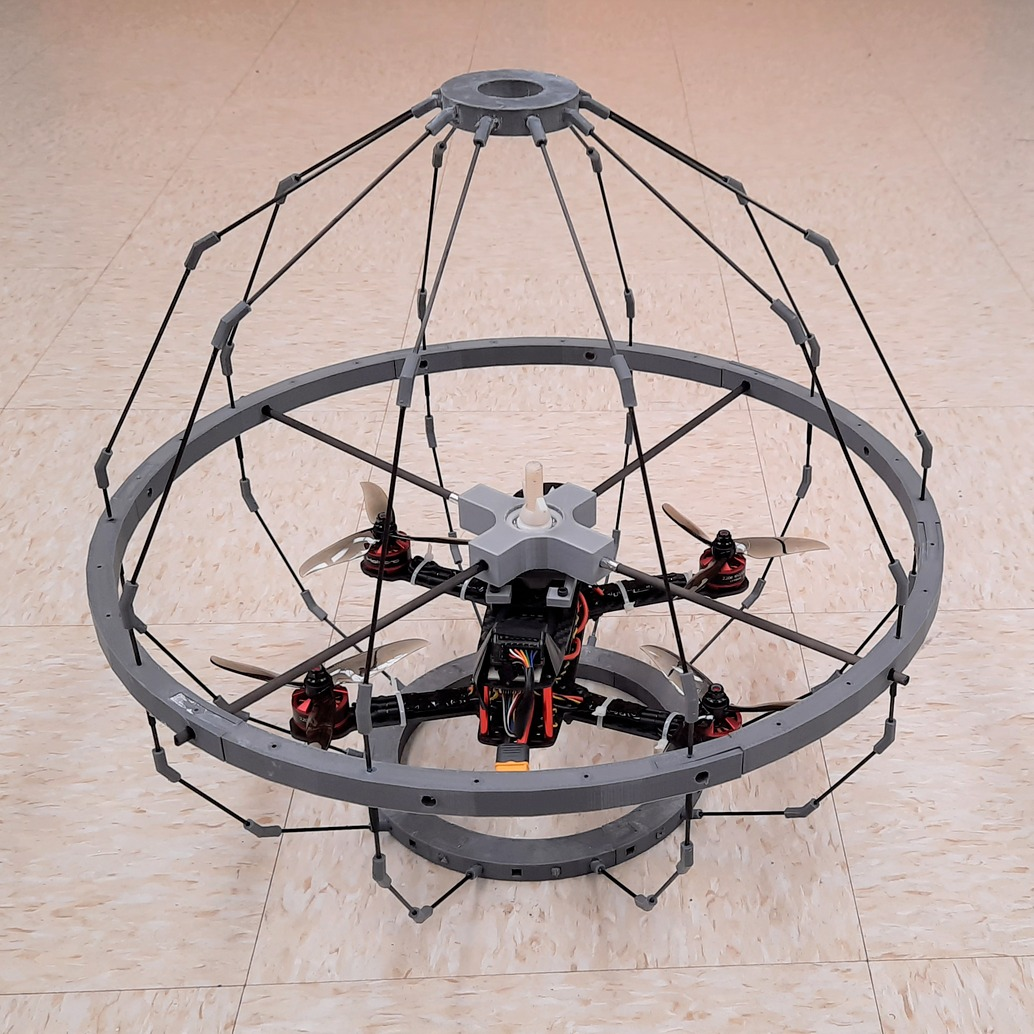
\includegraphics[width=\textwidth,height=4.5cm,keepaspectratio]{Figures/mahmud_turtle_cage.jpg}
        \caption{Mahmud's turtle-shell cage design. Adapted from~\cite{mahmudDevelopmentCollisionResilient2021}.}
        \label{fig:mahmud_turtle}
    \end{subfigure}
    \hfill
    \begin{subfigure}{0.48\textwidth}
        \centering
        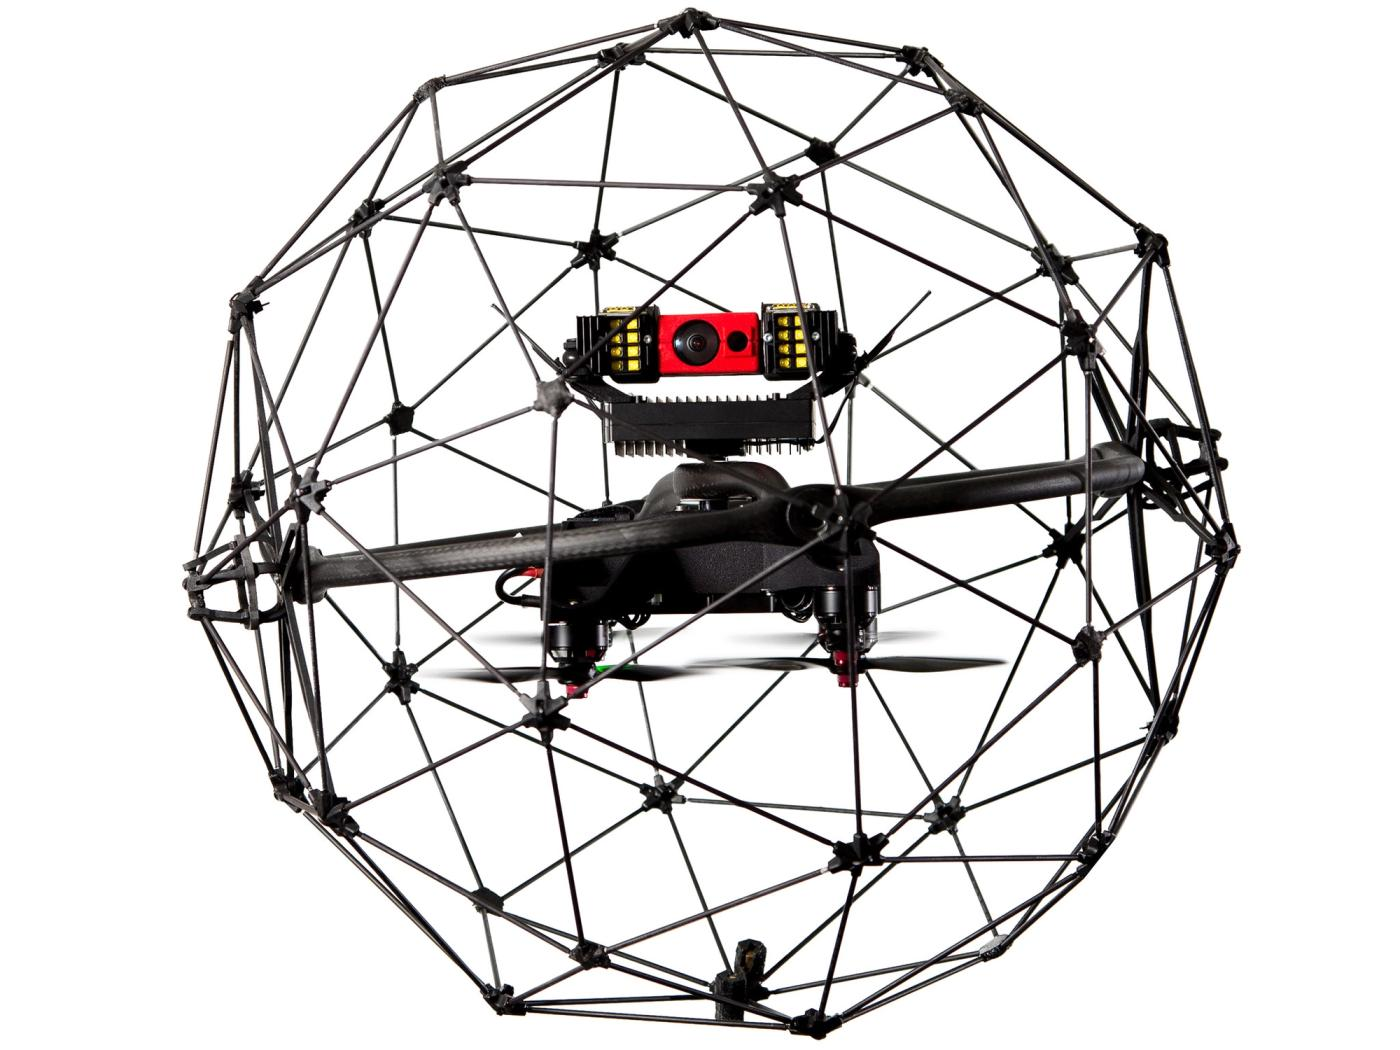
\includegraphics[width=\textwidth,height=4.5cm,keepaspectratio]{Figures/Elios_Flyability.jpg}
        \caption{Flyability Elios 3 inspection drone. Image: flyability.com.}
        \label{fig:elios}
    \end{subfigure}
    \caption{Collision-resilient cage designs in research and industry. (a)~Mahmud's single-axis turtle-shell cage demonstrating the rotating-shell principle; (b)~the commercially deployed Flyability Elios series confirming the practical viability of decoupled protective cages.}
    \label{fig:cage_designs}
\end{figure}

The rotating-cage concept has also reached commercial maturity in the Flyability Elios series~\cite{briod2014collision}, confirming the practical viability of decoupled protective cages for confined-space inspection.

Freely rotating spherical cages provide a distinct kinematic advantage during the \emph{airborne} impact itself: they convert linear collision momentum into rotational energy. This mechanism allows the cage to roll along a surface rather than scrape, mitigating the aggressive stick-slip friction dynamics that typically destabilise a drone's flight controller during sustained contact. This principle of kinetic impact deflection forms the mechanical baseline investigated in this thesis.

\subsection{Tactile Sensing and the IMU Noise Problem}

The concept of using physical contact as a sensing modality has precedent in robotics literature. In ground robotics, tactile whiskers and force-sensitive skins have long been used to map environments in low-visibility conditions. Extending this to aerial vehicles, the challenge is that contact events are highly transient and high-bandwidth, demanding both mechanical resilience to survive the impact and sufficient sensor fidelity to record meaningful data through the shock.

Currently, extracting this information from standard onboard sensors remains an open challenge. The dominant assumption in the literature is that standard commercial Inertial Measurement Units (IMUs) are unsuitable for accurate impact characterisation. Liu and Karydis~\cite{liuImpactresilientQuadrotorDesign2021} explicitly noted that the transient shockwaves of a collision overwhelm standard IMUs, rendering the data too noisy for reliable state estimation. To bypass this limitation, they equipped their Actively Resilient Quadrotor (ARQ) with custom Hall sensors mounted on prismatic shock absorbers to measure impact forces mechanically.

The combination of a deflection mechanism with onboard inertial measurement for angle inference, as pursued in this work, represents a novel intersection of these requirements. While traditional linear filtering struggles to extract meaningful collision geometry from chaotic IMU data, the noise generated by an impact is structurally dictated by the drone's collision mechanics. By applying a non-linear Random Forest regressor to these vibrational signatures, this thesis investigates whether the impact angle can be mathematically decoded from standard IMU data alone, potentially eliminating the need for specialised contact sensors in confined-space operations.
